\section{波导理论}

微波传输线是用来传输微波信号和微波能量的传输线。如第 2 章 2.1 节所介绍的那样,微波传输线的种类很多,比较常用的有平行双线、矩形波导、圆波导、同轴线、带状线和微带线等。一般根据不同的用途和工作频段选用不同类型的传输线。

在微波的低频段,可采用平行双线来传输微波电磁能量;但当频率提高后,平行双线会向空间辐射电磁能量,且频率愈高,能量损耗愈大。所以在微波的高频段,平行双线不能使用,一般采用同轴线和波导等类型的传输线,这类传输线是封闭式的,不存在辐射损耗。随着频率的继续提高,同轴线的横截面尺寸必须相应减小才能保证只传输 TEM 波,这样导致同轴线的导体损耗增加,功率容量下降。因此同轴线不能传输更高频率的电磁波,一般只适用于厘米波段。

对于更高频率的电磁波,可采用波导进行传输。波导是空心金属管,它传输的功率容量最大;但它的带宽较窄,体积和重量较大。随着空间技术的发展,对微波集成电路需要越来越多,显然同轴线和波导不能满足这种需要,所以出现了带状线和微带线等形式的传输线。特别是微带线,具有体积小、重量轻和频带宽等优点,是目前微波集成电路中采用最多的传输线。但它的缺点是功率容量小,损耗较大,所以主要用于小功率系统中。

微波传输线是引导电磁波沿一定方向传输的系统,故又称做导波系统。被传输的电磁波又称做导行波。导行波一方面要满足麦克斯韦方程,另一方面又要满足导体或介质的边界条件;也就是说,麦克斯韦方程和边界条件决定了导行波在导波系统中的电磁场分布规律和传播特性。

本章首先采用电磁场理论来分析矩形波导、圆波导和同轴线的传播特性和电磁场分布规律,然后借助传输线理论来分析带状线、微带线、耦合带状线和耦合微带线的基本特点和传输规律。



\subsection{交变电磁场基本关系式}

\textbf{场量的瞬时值与复数振幅值之间的关系为}
\[
E(x, y, z, t) = E(x, y, z) \cos(\omega t + \theta)
\]
\[
= \operatorname{Re}\left[\underline{E}(x, y, z) e^{j\theta} e^{j\omega t}\right] = \operatorname{Re}\left[\hat{E}(x, y, z) e^{j\omega t}\right]
\tag{3-1-1}
\]

\textbf{可得复数形式的麦克斯韦方程组为}
\[
\begin{aligned}
	\nabla \times \dot{E} &= -j \omega \mu \dot{H}, \\
	D &= \varepsilon E, \\
	B &= \mu H, \\
	\nabla \times \dot{H} &= j \omega \varepsilon \dot{E} + J, \\
	\nabla \cdot \dot{D} &= \rho, \\
	\nabla \cdot \dot{B} &= 0
\end{aligned}
\tag{3-1-2}
\]

一般都假定远离场源 $\rho = 0$, $J = 0$,即在无源区
\[
\begin{aligned}
	\nabla \times E &= -j \omega \mu H, \\
	\nabla \times H &= j \omega \varepsilon E, \\
	\nabla \cdot D &= 0, \\
	\nabla \cdot B &= 0.
\end{aligned}
\tag{3-1-3}
\]

\subsection{边界条件}

\begin{figure}[htbp]
	\centering
	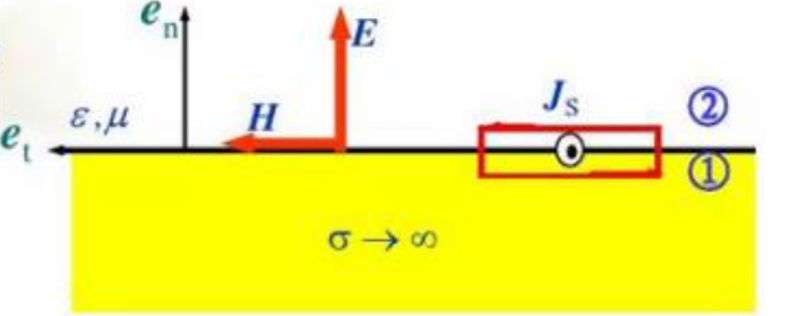
\includegraphics[width=0.4\textwidth]{img/3-5.png} % 图片文件名,不需要加扩展名
	\caption{边界条件示意图}
	\label{fig:example}
\end{figure}

\begin{equation}
	\begin{aligned}
		n \times (E_2 - E_1) &= 0 & \quad (E_{2t} - E_{1t}) &= 0 \\
		n \times (H_2 - H_1) &= J_s & \quad (H_{2t} - H_{1t}) &= 0 \\
		n \cdot (D_2 - D_1) &= \rho_s & \quad (D_{2n} - D_{1n}) &= 0 \\
		n \cdot (B_2 - B_1) &= 0 & \quad (B_{2n} - B_{1n}) &= 0
	\end{aligned}
	\tag{3-2-1}
\end{equation}

式中 $ n $ 为由媒质 1 指向媒质 2 的法向单位矢量,$ J_s $ 为界面上的电流密度,$ \rho_s $ 为界面上的面电荷密度。
$ n $:由媒质 1 指向媒质 2 的法向单位矢量;
$ J_s $:界面上的电流密度;
$ \rho_s $:界面上的面电荷密度。

在理想导体表面上,电场 $E_2$​总是垂直于表面,而磁场$ H_2​$总是平行于表面;电位移矢量 $D 2​$等于自由电荷面密度$ ρ s​$,并垂直于表面;在导体表面上的电流密度 $J s$等于表面的磁场强度$ H 2​$,其方向为 $n$× $H 2$ ,并可由右手定则确定。


\subsection{理想波导系统的一般理论}

理想导波系统一般指规则的金属波导管,分析时一般只讨论远离场源的区域,并常采用广义正交坐标系 $(u_1, u_2, z)$,其中 $u_1$ 和 $u_2$ 为波导横截面上的坐标,$z$ 为波导纵向坐标。导波系统中电场和磁场在广义正交坐标系中,可用其横向分量和纵向分量来表示
\begin{align*}
	\mathbf{E}(u_1, u_2, z) &= \mathbf{E}_T(u_1, u_2, z) + \mathbf{E}_z(u_1, u_2, z) = \mathbf{E}_T + \mathbf{E}_z 
	\tag{3-3-1}
	\\
	\mathbf{H}(u_1, u_2, z) &= \mathbf{H}_T(u_1, u_2, z) + \mathbf{H}_z(u_1, u_2, z) = \mathbf{H}_T + \mathbf{H}_z
	\tag{3-3-2}
\end{align*}
式中:$\mathbf{E}_T$ 和 $\mathbf{H}_T$——电场和磁场的横向分量;\\
$\mathbf{E}_z$ 和 $\mathbf{H}_z$——电场和磁场的纵向分量。

导波系统中的电磁波按纵向场分量的有无,可分为以下三种波型(或模):
\begin{enumerate}
	\item 横磁波(TM 波),又称电波(E 波):$\mathbf{H}_z = 0$, $\mathbf{E}_z \neq 0$;
	\item 横电波(TE 波),又称磁波(H 波):$\mathbf{E}_z = 0$, $\mathbf{H}_z \neq 0$;
	\item 横电磁波(TEM 波):$\mathbf{E}_z = 0$, $\mathbf{H}_z = 0$。
\end{enumerate}

其中横电磁波只存在于多导体系统中,它是非色散波;而横磁波和横电波一般存在于单导体系统中,它们是色散波。下面分别讨论上述三种波型的场量关系式。


\begin{table}[htbp]
	\centering
	\caption{三类波型的主要关系式}
	\label{tab:wave_relations}
	\begin{tabular}{c|c|c|c}
		\hline
		& TEM 波 & TM 波 & TE 波 \\
		\hline
		横向分布函数 & 拉普拉斯方程 & 亥姆霍兹方程 & 亥姆霍兹方程 \\
		& $\nabla^2 \phi = 0$ & $\nabla^2 \phi + k_c^2 \phi = 0$ & $\nabla^2 \psi + k_c^2 \psi = 0$ \\
		\hline
		相移常数 ($k > k_c$) & $\beta = k = \omega \sqrt{\mu \epsilon}$ & $\beta = \sqrt{k^2 - k_c^2}$ & $\beta = \sqrt{k^2 - k_c^2}$ \\
		& & $k = \omega \sqrt{\mu \epsilon}$ & $k = \omega \sqrt{\mu \epsilon}$ \\
		\hline
		广义传输线方程 & $\frac{\mathrm{d}U(z)}{\mathrm{d}z} = -j \omega \mu I(z)$ & $\frac{\mathrm{d}U(z)}{\mathrm{d}z} = \frac{1}{j \omega \epsilon} (k^2 - k_c^2) I(z)$ & $\frac{\mathrm{d}I(z)}{\mathrm{d}z} = -j \omega \mu U(z)$ \\
		& $\frac{\mathrm{d}I(z)}{\mathrm{d}z} = -j \omega \epsilon U(z)$ & $\frac{\mathrm{d}I(z)}{\mathrm{d}z} = -j \omega \epsilon U(z)$ & $\frac{\mathrm{d}I(z)}{\mathrm{d}z} = \frac{1}{j \omega \mu} (k^2 - k_c^2) U(z)$ \\
		\hline
		纵向场分量 & $E_z = H_z = 0$ & $E_z = \boldsymbol{\alpha}_z \frac{I(z)}{j \omega \epsilon} k_c^2 \phi$ & $H_z = \boldsymbol{\alpha}_z \frac{U(z)}{j \omega \mu} k_c^2 \psi$ \\
		\hline
		横向场分量 & $E_T = -U(z) \nabla_T \phi$ & $E_T = -U(z) \nabla_T \phi \times \boldsymbol{\alpha}_z$ & $E_T = -U(z) \nabla_T \psi \times \boldsymbol{\alpha}_z$ \\
		& $H_T = I(z) \nabla_T \phi \times \boldsymbol{\alpha}_z$ & $H_T = I(z) \nabla_T \phi \times \boldsymbol{\alpha}_z$ & $H_T = I(z) \nabla_T \psi$ \\
		\hline
		波阻抗 & $Z_{\text{TEM}} = \eta = \sqrt{\frac{\mu}{\epsilon}}$ & $Z_{\text{TM}} = \frac{\beta}{\omega \epsilon} = \frac{\sqrt{\omega^2 \mu \epsilon - k_c^2}}{\omega \epsilon}$ & $Z_{\text{TE}} = \frac{\omega \mu}{\beta} = \frac{\omega \mu}{\sqrt{\omega^2 \mu \epsilon - k_c^2}}$ \\
		\hline
	\end{tabular}
\end{table}

\subsection{导波系统的传输特性}

1. “高通低不通”
→ 高通滤波器

2. 多模
理论上,在矩形波导中能存在着无穷多个 $TE_{mn} $、$ TM_{mn} $模式,它们都满足波动方程并能满足矩形波导的边界条件。

3. 主模
在波导中,通常称截止波长最大(对应截止波数或截止频率最小)的模式为主模,也称基模或最低模式。而将其他为实现单一 TE 10​模传输,必须满足下列条件:
\[
(\lambda_c)_{H_{10}} = 2a > \lambda > \max \left\{ (\lambda_c)_{H_{20}} = a, (\lambda_c)_{H_{01}} = 2b \right\}
\tag{3-4}
\]
4. 简并截止波数$ ( k_c )$或截止波长 $( \lambda_c )$、截止频率 $( f_c )$相同但场分布不同的模式称为“简并”模式。

5. 色散
相速度随频率变化的现象称为色散。

6. 完备性
由三角函数的完备性,可以证明,矩形波导中所有可能存在的导波场结构都可以用 $TE_{mn} $、$ TM_{mn} $模的线性组合来表示。

\subsection{矩形波导中电磁波型的传输特性}
虽然矩形波导中可能存在无限多的 TE 和 TM 波型,但哪些波型能够在波导中传输,还取决于工作频率和波导尺寸。合理地选择工作频率和波导尺寸,可以使需要的波型能传输,而使不需要的波型截止掉。


截止波长不仅与波导尺寸 a 和 b 有关,而且与决定波型的 m 和 n 有关。不同的 m 、n 值代表不同的波型,具有不同的场分布;但对同一组 m 、 n 值,TE 波和 TM 波有相同的截止波长(频率),即 (λ c​) TM mn​=(λ c​) TE mn​。这种截止波长(频率)相同而场分布不同的一对波型称为“简并波”。矩形波导中的波型一般都是简并的波型,但 TE m0
​和 TE 0n​是非简并波,因为矩形波导中不存在 TM m0​波和 TM 0n​波。

当波导尺寸 a 和 b 给定时,将不同 m 和 n 值代入式 (3-5-12a) 中,即可得到不同波型的截止波长。例如,对于常用 BJ-100 型波导,其标称尺寸为 a×b=22.86mm×10.16mm,故可计算出各波型的 λ c​值,其分布如图 3-5-2 所示。



\begin{figure}[htbp]
	\centering
	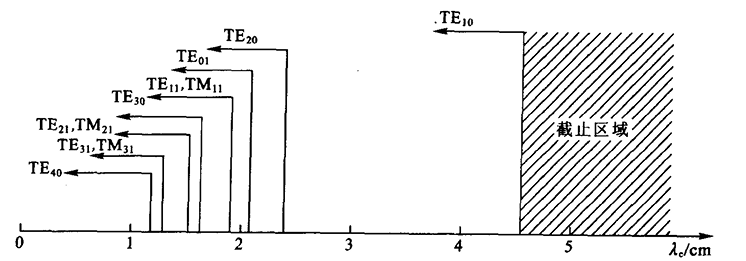
\includegraphics[width=0.7\linewidth]{img/3-6}
	\caption{识别文字BJ-100型波导不同波型截止波长的分布图}
	\label{fig:3-6}
\end{figure}

从图中可以看出,TE({10})模的截止波长最长,它右边的阴影区为截止区。

(1) 当工作波长 λ=5 cm 时,波导对所有的波型都截止,此时的波导称为“截止波导”。

(2) 当 λ=4 cm 时,波导只能传输 TE 10​
模,此时的波导称为“单模波导”。

(3) 当 λ=1.5 cm 时,波导可同时传输 $TE_{10}$、$TE_{20}$、$TE_{01}$、$TE_{11} $、$TM_{11}$ 及 $TE_{30}$等波型,此时的波导称为“多模波导”。

\subsection{圆波导中的三种主要模式}
圆波导中有无限多个模式存在,最常用的三个主要模式为 $TE_{11} $、$ TE_{01}$ 和 $TM_{01}$模。下面分别介绍这三种模式的特点和它们的应用。

\subsubsection{TE 11模 (λc= 3.41R)}

TE 11​模的场分布如图 6 所示。其中图 6(a) 表示横截面上的电磁场分布;图 6(b) 表示纵剖面上的电场分布;图 6(c) 表示圆波导壁上的壁电流分布。

\begin{figure}[htbp]
	\centering
	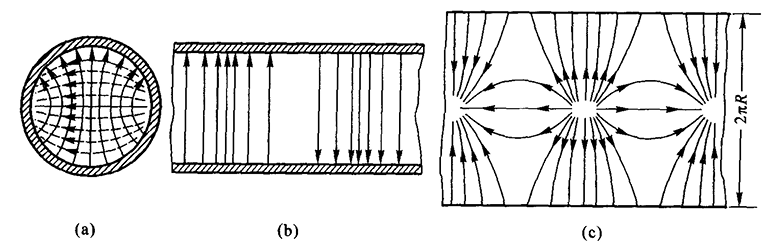
\includegraphics[width=0.7\linewidth]{img/3-6-1}
	\caption{$TE_{11}$模场分布图}
	\label{fig:3-6-1}
\end{figure}

由图可见,圆波导中 TE 11​模的场分布和矩形波导中 TE 10​模的场分布很相似,因此圆波导中 TE 11​模很容易通过矩形波导中 TE 10​模过渡得到,而且 TE 11​模的截止波长最长,容易实现单模传输。因此,圆波导的极化衰减器、波型变换器和铁氧体环行器均采用 TE 11​模作为工作模式。但由于 TE 11​模存在极化简并模,故不宜用来作为远距离传输的工作模式。

\subsubsection{ $TE_{01}$模 (λc=1.64R)}

$TE_{01}$模的场分布如图 7 所示。其中图 7(a) 表示横截面上的电磁场分布;图 7(b) 表示纵剖面上的电磁场分布;图 7(c) 表示壁电流分布。

\begin{figure}[htbp]
	\centering
	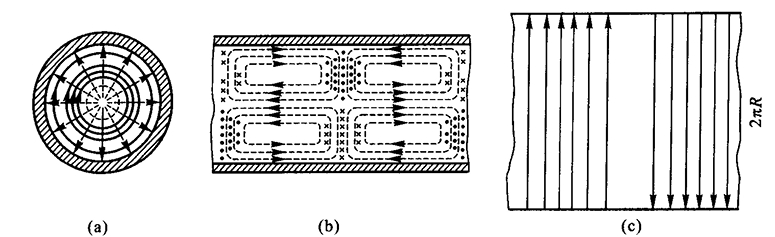
\includegraphics[width=0.7\linewidth]{img/3-6-2}
	\caption{$TE_{01}$模场分布图}
	\label{fig:3-6-2}
\end{figure}

由图可见,TE 01​模的电场只存在 E φ​分量,且在 r=0 和 R 处,$ E_varphi = 0 $;在波导壁上只有磁场的  $H_z$ 分量,故在壁上只有 J φ电流,且随频率的升高而减小,从而 TE 01​模的导体损耗随频率升高而降低。因此,TE 01模常作为高 Q 谐振腔和远距离的毫米波传输线的工作模式。另外由于它是圆电模,也可作为连接元件和天线馈线系统的工作模式。但由于它不是主模,因此该模式作为工作模式时,必须设法抑制其他模式。

\subsubsection{ $TM_{01}$模 (λc=1.64R)} 
TM 01模的场分布如图 8 所示。其中图 8(a) 表示横截面上的电磁场分布;图 8(b) 表示纵剖面上的电磁场分布;图 8(c) 表示壁电流的分布。

\begin{figure}[htbp]
	\centering
	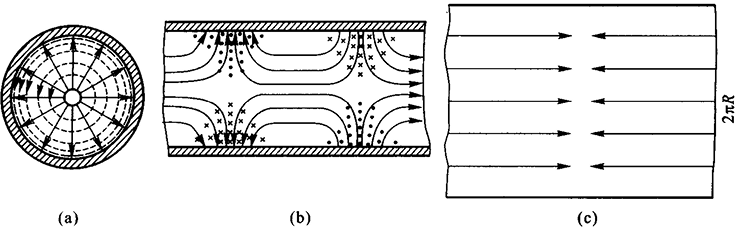
\includegraphics[width=0.7\linewidth]{img/3-6-3}
	\caption{$TM_{01}$模场分布图}
	\label{fig:3-6-3}
\end{figure}

由图可见,TM 01​模的磁场只有 H φ​分量,是具有轴对称分布的圆磁场;电场只有 E z分量,且在 r=0 处 E z​最大;壁电流只有纵向分量 J z​。因此适用于微波天线馈线旋转铰链的工作模式。由于它具有 E z分量,便于和电子交换能量,可做电子直线加速器的工作模式。但由于它的管壁电流具有纵向电流,故必须采用抗流结构的连接方式。






